% ---
% Figuras complementarias del Análisis Exploratorio de Datos (Capítulo 4).
% Decisiones y hallazgos que lo respaldan: D-005, D-006, D-009, D-022, H-001, H-002, H-050.
% ---

\subsection{Figuras del análisis exploratorio}
\label{anx:figuras_eda}

Las siguientes figuras complementan la caracterización realizada en el
capítulo~\ref{sec:eda}, reuniendo aquellas distribuciones de clases,
metadatos clínicos, características de escáner e intensidades de píxeles
trasladadas del cuerpo principal para optimizar la concisión del reporte técnico.

\begin{figure}[htbp]
  \centering
  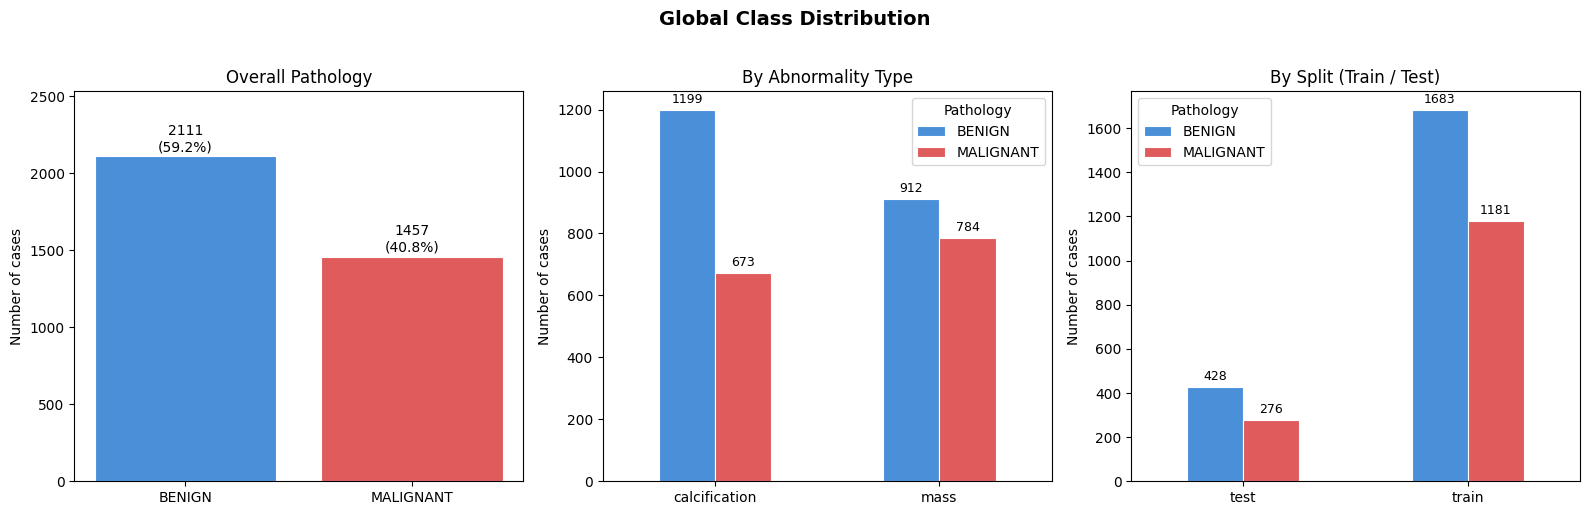
\includegraphics[width=\textwidth]{Figures/B1_class_distribution.png}
  \caption{Distribución de clases global, por tipo de hallazgo y por split train/test.}
  \label{fig:class_distribution}
\end{figure}

\begin{figure}[htbp]
  \centering
  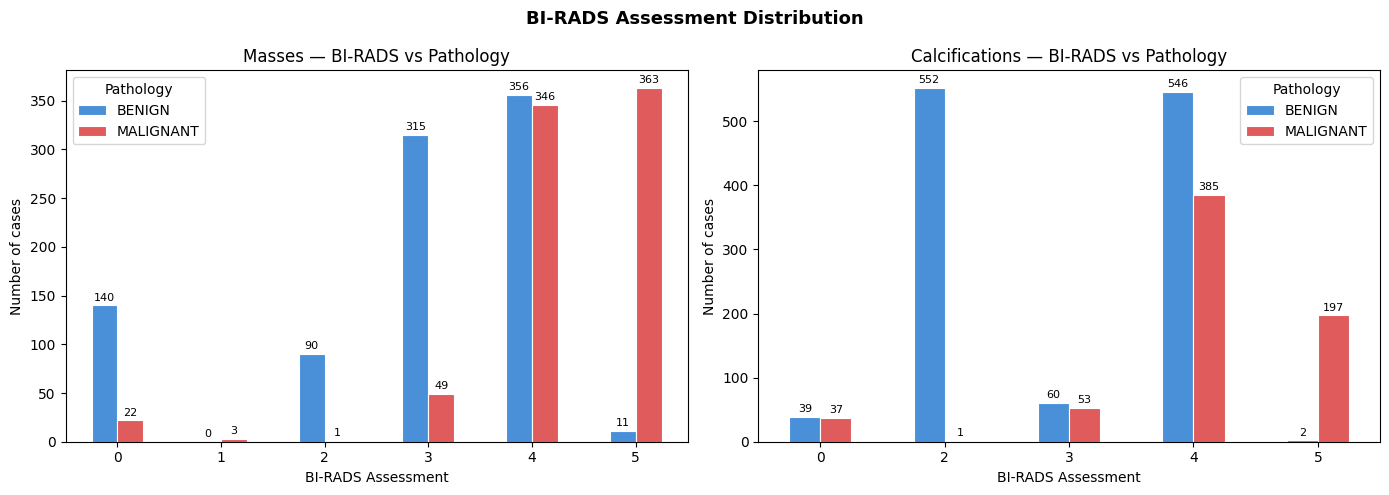
\includegraphics[width=\textwidth]{Figures/B3_birads_distribution.png}
  \caption{Distribución de categorías BI-RADS por patología y tipo de hallazgo.}
  \label{fig:birads_distribution}
\end{figure}

\begin{figure}[htbp]
  \centering
  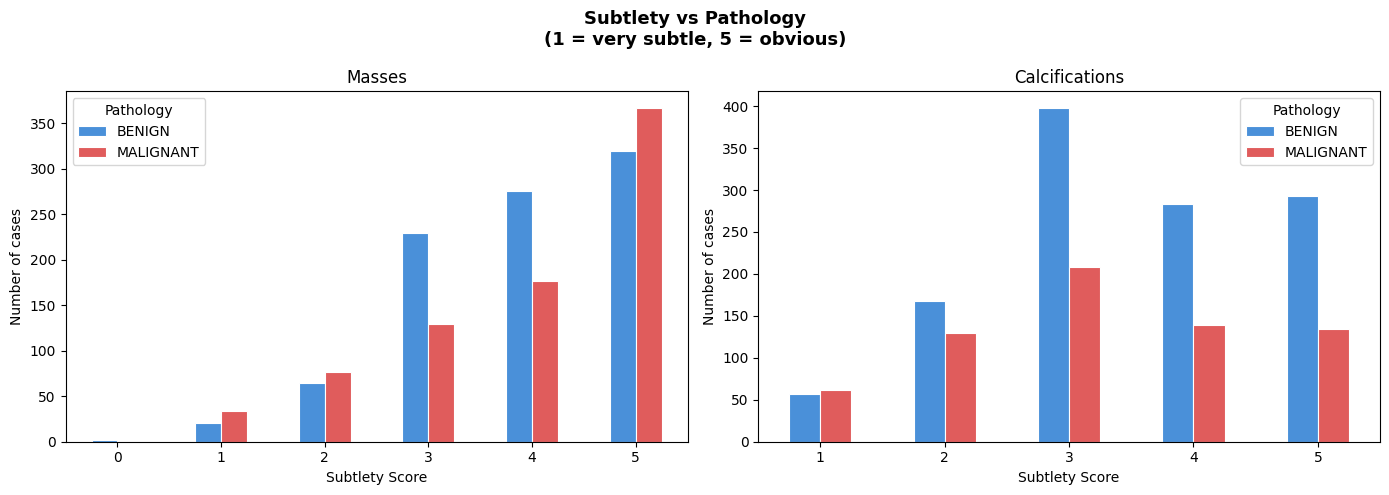
\includegraphics[width=\textwidth]{Figures/B4_subtlety_distribution.png}
  \caption{Distribución de \textit{subtlety} por patología y tipo de hallazgo (1\,=\,muy sutil, 5\,=\,obvio).}
  \label{fig:subtlety_distribution}
\end{figure}

\begin{figure}[htbp]
  \centering
  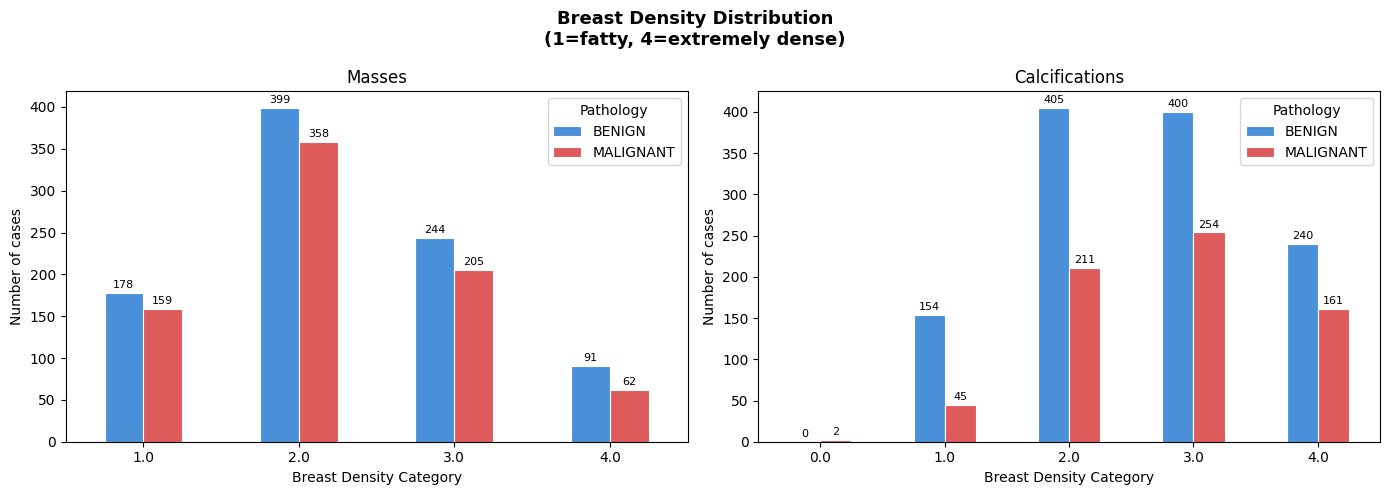
\includegraphics[width=\textwidth]{Figures/C1_breast_density.png}
  \caption{Distribución de densidad mamaria (1\,=\,grasa, 4\,=\,extremadamente densa) por patología y tipo de hallazgo.}
  \label{fig:breast_density}
\end{figure}

\begin{figure}[htbp]
  \centering
  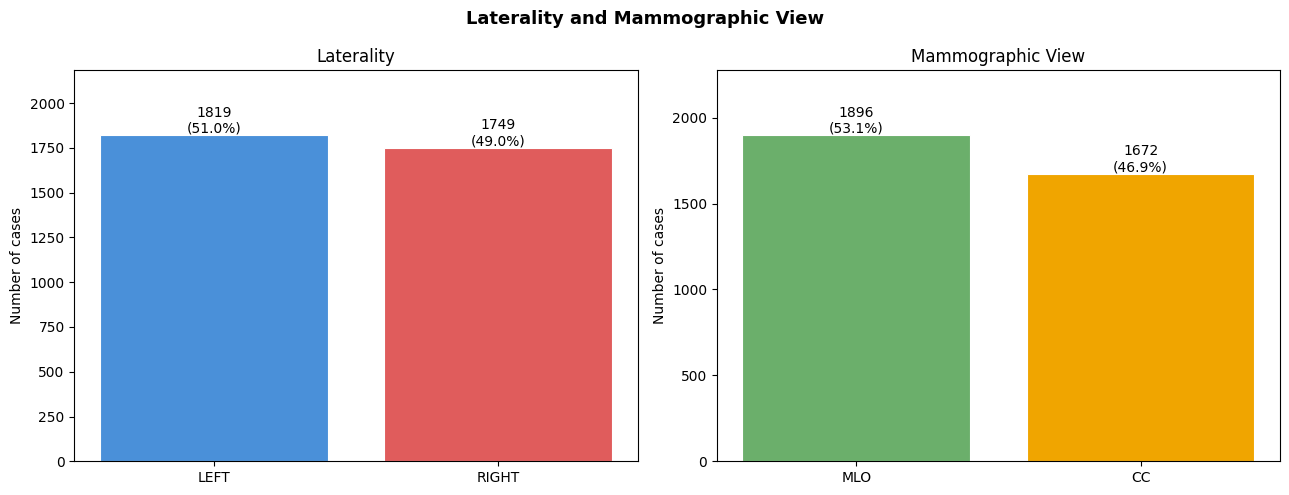
\includegraphics[width=\textwidth]{Figures/C2_laterality_view.png}
  \caption{Distribución de lateralidad y vista mamográfica en el dataset.}
  \label{fig:laterality_view}
\end{figure}

\begin{figure}[htbp]
  \centering
  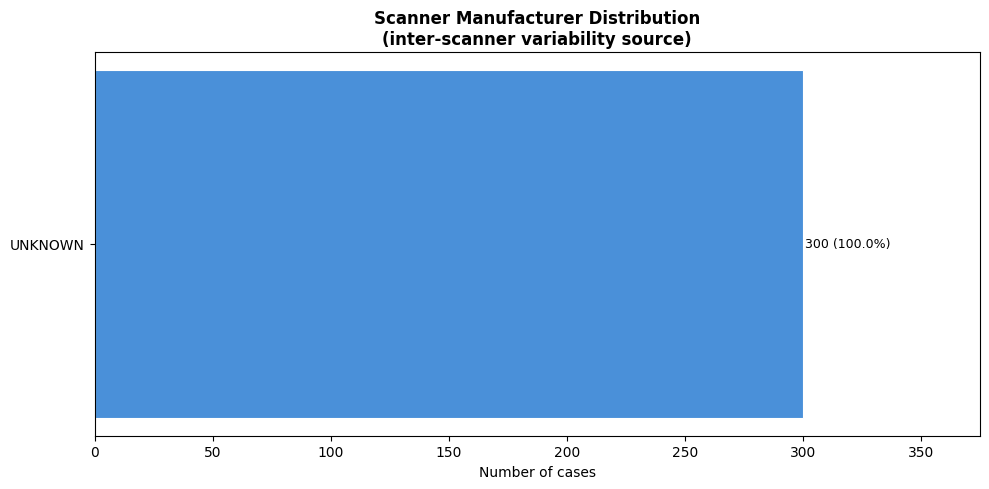
\includegraphics[width=0.8\textwidth]{Figures/D2_manufacturers.png}
  \caption{Distribución de fabricantes de escáner en la muestra analizada.}
  \label{fig:manufacturers}
\end{figure}

\begin{figure}[htbp]
  \centering
  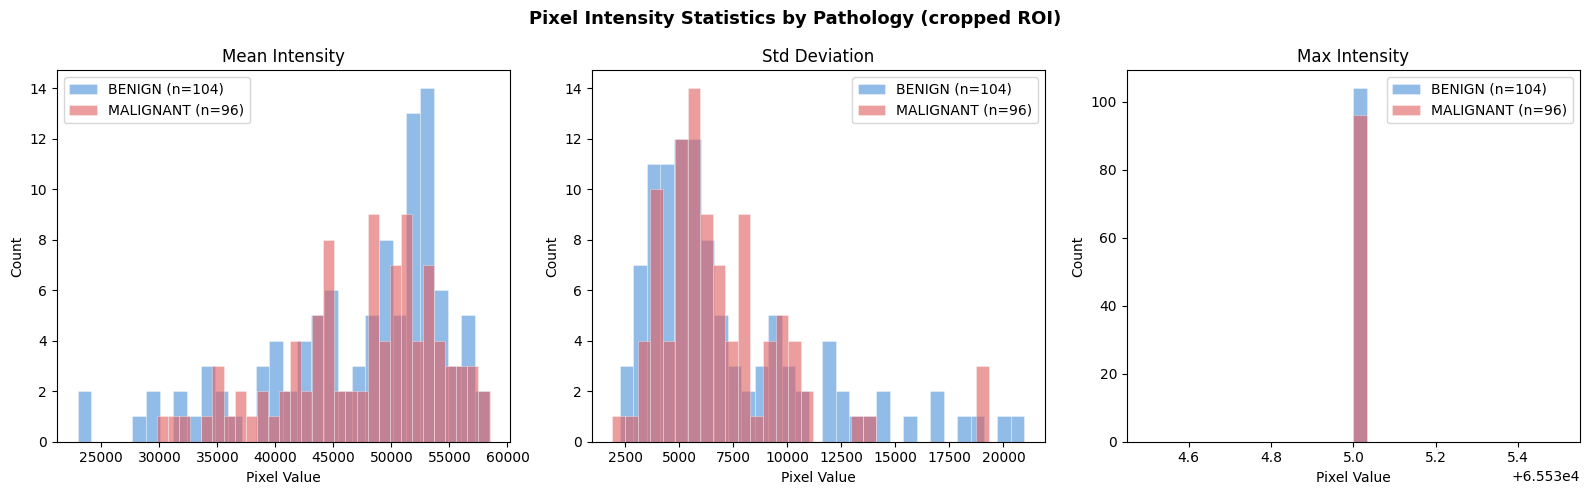
\includegraphics[width=\textwidth]{Figures/D3_pixel_intensities.png}
  \caption{Distribución de estadísticas de intensidad de píxeles (media, desviación estándar y máximo) en imágenes recortadas de ROI, por patología.}
  \label{fig:pixel_intensities}
\end{figure}

\begin{figure}[htbp]
  \centering
  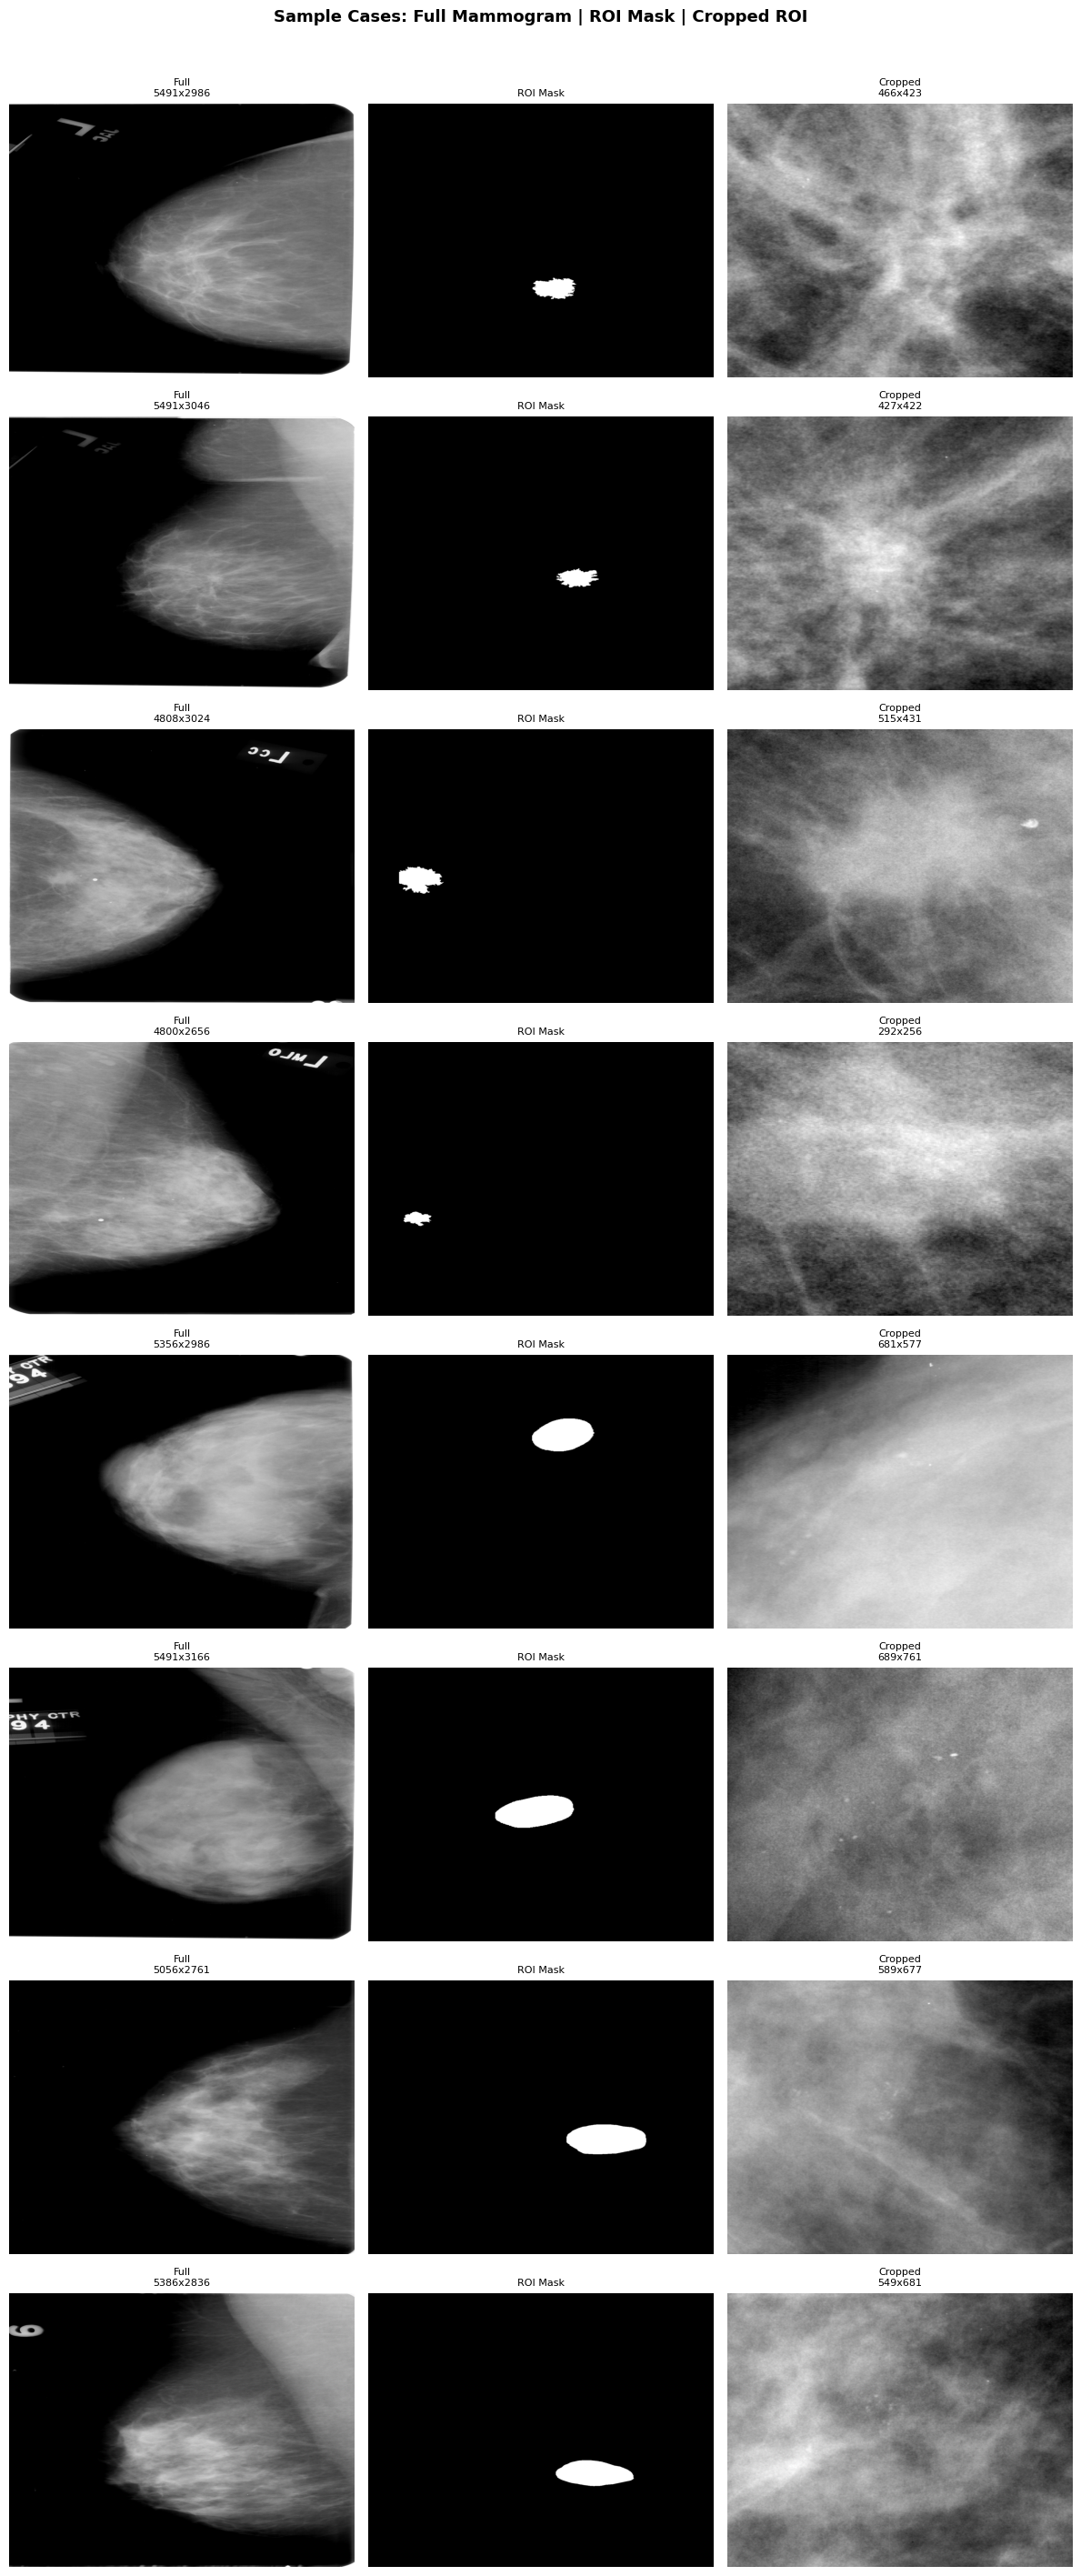
\includegraphics[width=0.7\textwidth, height=0.72\textheight, keepaspectratio]{Figures/D4_sample_gallery.png}
  \caption{Galería de casos representativos: mamografía completa, máscara ROI e imagen recortada, para masas y calcificaciones benignas y malignas.}
  \label{fig:sample_gallery}
\end{figure}
